\begin{question}{18}{
    Het Commando Landstrijdkrachten (CLAS) test een nieuw type accu voor draagbare communicatiemiddelen.
    De fabrikant claimt een gemiddelde gebruiksduur van $\mu_0 = 36$ uur per volledig opgeladen accu.
    Uit eerdere productreeksen is bekend dat de gebruiksduur normaal verdeeld is met een \emph{bekende} standaardafwijking van $3.0$ uur.
    Een testpartij van $n = 25$ accu's geeft een steekproefgemiddelde van $34.6$ uur.
}

    \subquestion{6}{
        Bereken een tweezijdig \SI{96}{\percent}-betrouwbaarheidsinterval voor de gemiddelde gebruiksduur $\mu$ op basis van de gegeven steekproefdata.
        Rond de grenzen af op één decimaal, zodanig dat de betrouwbaarheid gewaarborgd blijft.
        Is er reden om aan te nemen dat de gemiddelde gebruiksduur significant afwijkt van $36$ uur?
    }

    \solution{
        In de vraag is gegeven dat $\mu_0 = 36$ uur, het steekproefgemiddelde
        $\samplemeanx = 34.6$ uur, de populatiestandaardafwijking
        $\sigma = 3.0$ uur en de steekproefgrootte $n = 25$.

        De gebruiksduur $X$ van een willekeurige accu is normaal verdeeld met $\mu = \text{ ?}$ en $\sigma = 3.0$. 
        We willen een betrouwbaarheidsinterval voor de onbekende $\mu$ berekenen op basis van de steekproefgegevens. 
        
        Omdat de standaardafwijking $\sigma$ bekend is, mogen we een betrouwbaarheidsinterval bepalen met behulp van de normale verdeling.\rubric{1}
        
        Verder is $\alpha = 0.04$, omdat we een \SI{96}{\percent}-betrouwbaarheidsinterval willen berekenen.
        De bijbehorende $z$-waarde is gelijk aan
        \[
            z_{\alpha/2} = \invnorm(\opp=1-\frac{\alpha}{2}=0.98, \mu=0, \sigma=1) \approx 2.0537.\rubric{1}
        \]
        Het \SI{96}{\percent}-betrouwbaarheidsinterval wordt dan gegeven door
        \begin{align*}
            &\phantom{=}[\samplemeanx - z_{\alpha/2} \cdot \frac{ \sigma }{ \sqrt{ n } }, \samplemeanx + z_{\alpha/2} \cdot \frac{ \sigma }{ \sqrt{ n } }] \\
            &= [34.6 - 2.0537 \cdot \frac{ 3.0 }{ \sqrt{ 25 } }, 34.6 + 2.0537 \cdot \frac{ 3.0 }{ \sqrt{ 25 } }] \\
            &= [33.3678, 35.8322].\rubric{2}
        \end{align*}
        Om de betrouwbaarheid te waarborgen, moeten we het interval naar buiten afronden, 
        oftewel op één decimaal afgerond krijgen we een interval van $[33.3, 35.9]$ uur. \rubric{1}

        Omdat de oorspronkelijke waarde $\mu_0 = 36$ uur niet in het betrouwbaarheidsinterval ligt, is er voldoende reden om aan te nemen dat de gemiddelde gebruiksduur significant afwijkt van $36$ uur.
        Specifiek is er voldoende reden om aan te nemen dat de gemiddelde gebruiksduur significant lager is dan $36$ uur.\rubric{1}
    }

    \subquestion{4}{
        De fabrikant wil de gemiddelde gebruiksduur nauwkeuriger schatten, namelijk met een maximale afwijking van $\pm 0.5$ uur bij \SI{96}{\percent} betrouwbaarheid.
        Wat is de minimaal benodigde steekproefomvang $n$ om met deze nauwkeurigheid te kunnen schatten?
    }

    \solution{
        Omdat de populatiestandaardafwijking $\sigma = 3.0$ bekend is, kunnen we gebruik maken van de volgende formule
        voor de minimaal benodigde steekproefomvang $n$ om een \SI{96}{\percent}-betrouwbaarheidsinterval te bepalen met afwijking $a = 0.5$:
        \[
            n \geq \left( \frac{z_{\alpha/2} \cdot \sigma}{a} \right)^2. \rubric{1}
        \]
        Invullen van de gegeven informatie geeft:
        \begin{align*}
            n   &\geq \left( \frac{z_{\alpha/2} \cdot \sigma}{a} \right)^2 \\
                &= \left( \frac{2.0537 \cdot 3.0}{0.5} \right)^2 \\
                &\approx 151.8438. \rubric{1}
        \end{align*}
        Aangezien de steekproefomvang $n$ een geheel getal moet zijn en we met grotere $n$ steeds nauwkeuriger kunnen schatten met dezelfde betrouwbaarheid,
        moeten we dit antwoord afronden naar boven. \rubric{1}

        We hebben dus minstens $n = 152$ accu's nodig. \rubric{1}
    }

    \subquestion{8}{
        CLAS is niet tevreden over de kwaliteit van de accu's van deze leverancier, en doet daarom een bestelling bij een tweede leverancier.
        Er worden voor een test $n = 36$ accu's bij deze nieuwe leverancier besteld.
        Van deze steekproef wordt bepaald dat de gemiddelde gebruiksduur gelijk is aan $35.5$ uur.
        Neem aan dat we nog steeds mogen werken met dezelfde \emph{bekende} standaardafwijking van $3.0$ uur. 
        
        CLAS is vooral geïnteresseerd in de vraag of de accu's gemiddeld \emph{korter} meegaan dan $36$ uur.
        Voer hiervoor een geschikte hypothesetoets uit met behulp van het kritieke gebied.
        Gebruik een significantieniveau $\alpha = 0.04$.
    }

    \solution{
        \subsubsection*{Stap 1: formuleer de nulhypothese $H_0$ en de alternatieve hypothese $H_1$.}
        Bij een toets of het gemiddelde $\mu$ van een normale verdeling kleiner is dan $\mu_0=36$ gebruiken we de volgende hypotheses
        \begin{align*}
            H_0: \quad \mu \geq 36\\
            H_1: \quad \mu < 36 \rubric{1}
        \end{align*}

        \subsubsection*{Stap 2: bepaal het significantieniveau $\alpha$.}
        Er is in de vraag gegeven dat we mogen werken met een significantieniveau $\alpha=0.04$.
        
        \subsubsection*{Stap 3: verzamel data voor het berekenen van de toetsingsgrootheid.}
        Ook is er in de vraag al steekproefdata verzameld voor de populatie accu's van de tweede leverancier, namelijk
        $\overline{x} = 35.5$. 

        \subsubsection*{Stap 4: bereken de toetsingsgrootheid.}
        De theoretische toetsingsgrootheid (hoofdletter!) bij een $z$-toets ($\sigma = 3.0$ is bekend!) is gelijk aan het steekproefgemiddelde $\overline{X}$. \rubric{1}
    
        Deze toetsingsgrootheid volgt onder $H_0$ een normale verdeling met $\mu = 36$ en $\sigma = \frac{3.0}{\sqrt{36}} = 0.5$. \rubric{1}
        
        De geobserveerde toetsingsgrootheid (kleine letter!) is gelijk aan $\overline{x} = 35.5$.
        
        \subsubsection*{Stap 5: bepaal de toetsuitslag (met behulp van het kritieke gebied).}

        Aangezien we een linkszijdige toets uitvoeren, is het kritieke gebied van de vorm $(-\infty, g)$, waarbij
        \[
            g = \invnorm(\opp=\alpha=0.04, \mu=36, \sigma=0.5) \approx 35.1247.
        \]        
        Het kritieke gebied is dus gelijk aan $(-\infty, 35.1247)$. \rubric{3}

        De geobserveerde toetsingsgrootheid $x = 35.5$ ligt niet in het kritieke gebied,
        dus we besluiten om $H_0$ niet te verwerpen.\rubric{1}

        \subsubsection*{Stap 6: vertaal de toetsuitslag terug naar de originele context van het probleem.}
        Er is onvoldoende reden om op basis van deze steekproef aan te nemen dat de gemiddelde gebruiksduur $\mu$
        van accu's van de tweede leverancier significant kleiner dan $36$ uur is.\rubric{1}
        \begin{center}
            \resizebox{0.9\textwidth}{!}{
                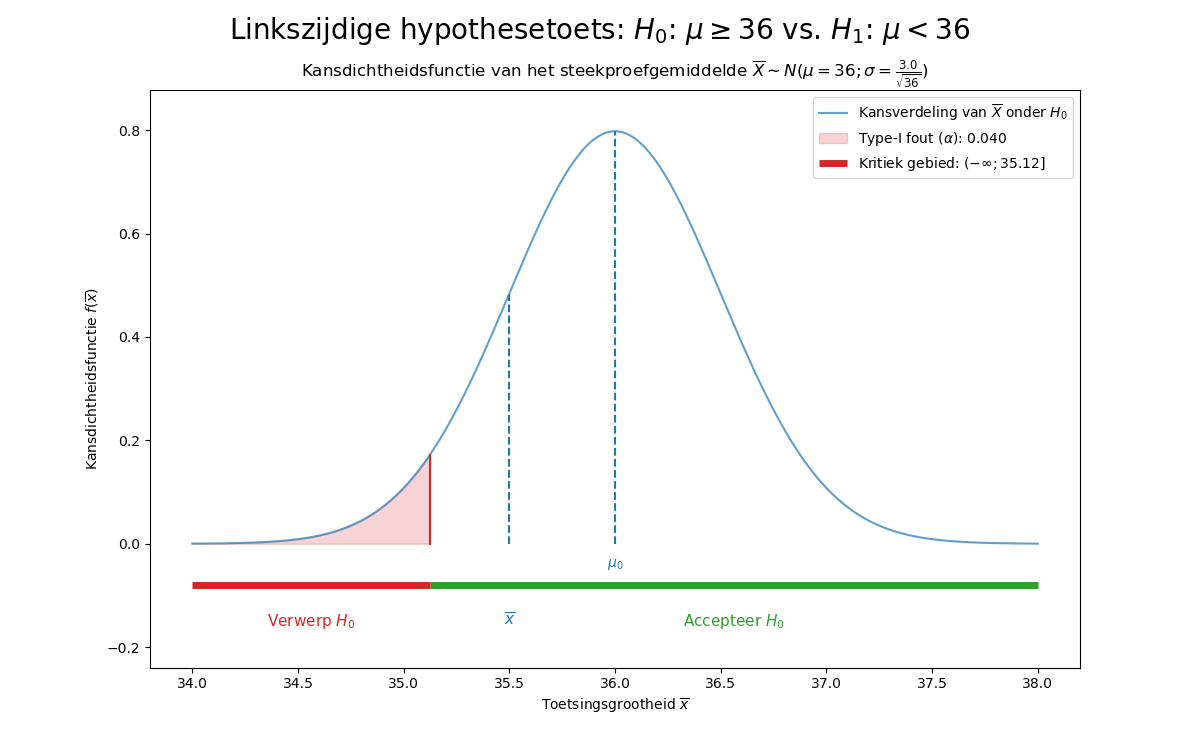
\includegraphics{../../LaTeX/figures/exam20261106_q1c.png}
            }
        \end{center}
    }

\end{question}
